\documentclass{article}

\usepackage[dutch]{babel}
\usepackage[margin=3cm]{geometry}
\usepackage{graphicx}
\usepackage{float}
\usepackage{caption}
\usepackage{hyperref}
\usepackage{amsmath}
\usepackage{wrapfig}
\usepackage[parfill]{parskip}

% fonts
\usepackage[T1]{fontenc}
\usepackage{helvet}
\renewcommand{\familydefault}{\sfdefault}

\graphicspath{{img/}}
 
\newcommand{\bold}[1]{\textbf{#1}}

\usepackage{minted}
\usepackage{upquote}
\usepackage{color}

\begin{document}

\begin{titlepage}
    \author{Tuur Vanhoutte}
    \title{Big Data}
\end{titlepage}

\pagenumbering{gobble}
\maketitle
\newpage
\tableofcontents
\newpage

\pagenumbering{arabic}

\section{Understanding Data Intensive Applications}

\subsection{Why Big Data?}

\subsubsection{Use case: data intensive application RouteYou}

\begin{figure}[H]
    \centering
    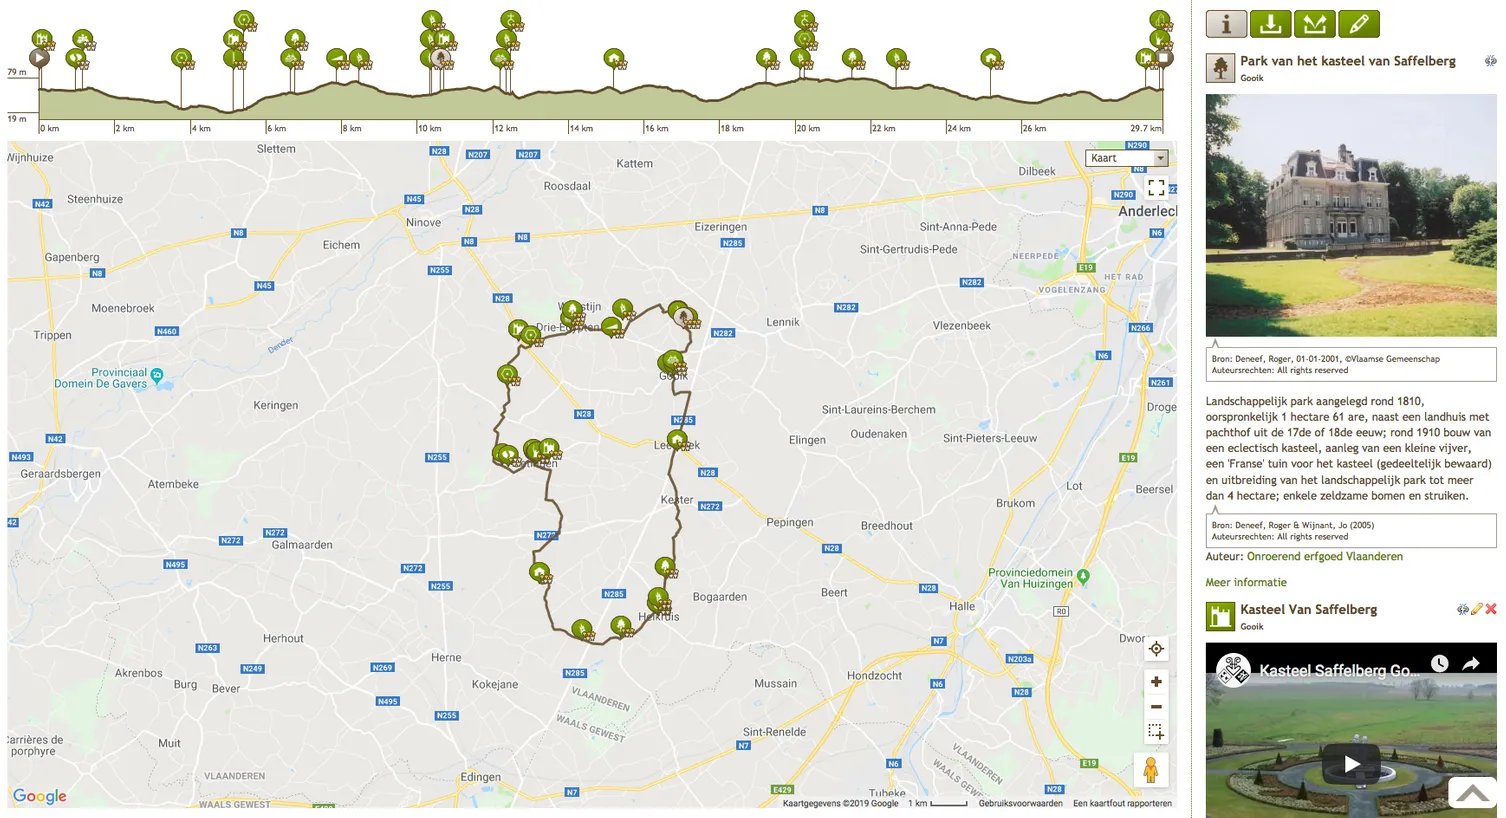
\includegraphics[width=0.5\textwidth]{routeyou.png}
    \caption{RouteYou}
\end{figure}

\begin{itemize}
    \item Routes - user preferences \& interests
    \item Searcheable Text data
    \item Geospatial data
    \item Community driven
    \begin{itemize}
        \item Exponential user growth is necessary to make the application posssible
        \item Server power/bills should grow linearly
    \end{itemize}
\end{itemize}

\subsection{Data Intensive Application: RAMS!}

\begin{itemize}
    \item \bold{Reliable}
    \begin{itemize}
        \item tolerating human mistakes
    \end{itemize}
    \item \bold{Available}
    \item \bold{Maintainable}
    \begin{itemize}
        \item Easy to adapt (evolvability)
        \item Easy to deploy \& operate (operations/sys admins)
    \end{itemize}
    \item \bold{Scalable}
    \begin{itemize}
        \item User growth while maintaining low response times
    \end{itemize}
\end{itemize}

\subsubsection{Common similar abbreviations}

\begin{itemize}
    \item Infrastructure: RAS (Reliable, Available, Serviceable)
    \item Developer: RMS (Reliable, Maintainable, Scalable)
\end{itemize}

\subsubsection{Methods to improve Maintainability}

\begin{itemize}
    \item Github
    \item Error handling
    \item Relative paths (not absolute)
    \item Abstraction (REST API, \dots)
    \item Documentation
\end{itemize}

\subsubsection{RAMS applied to RouteYou application}

\begin{itemize}
    \item Geospatial data (longitude, latitude)
    \item Available \& scalable
    \item Scalable \& low response time
    \item Community driven - unstructured text
    \item Maintainable: automatic classification of community input (ML)
\end{itemize}

\begin{figure}[H]
    \centering
    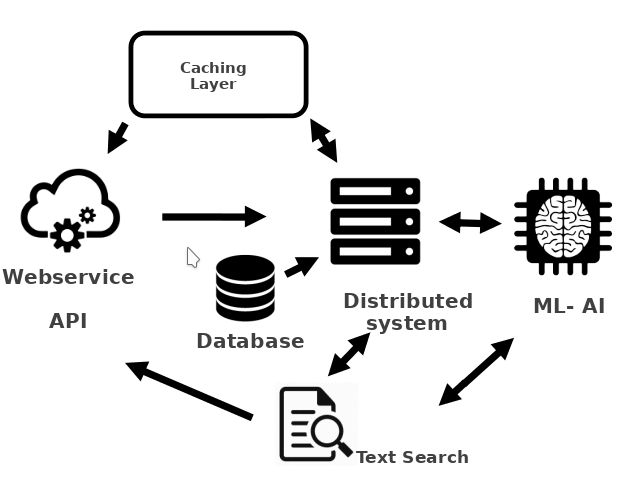
\includegraphics[width=0.5\textwidth]{RAMS-routeyou.png}
    \caption{To support many users, you need a caching layer}
\end{figure}


\subsection{Learning outcome for this module}

Being able to make infrastructure \& software choices to 
build a Reliable, Available, Maintainable \& Scalable (RAMS) 
data intensive application.

\begin{itemize}
    \item Deep insights into database technology \& cloud services
    \item Connecting with Machine Learning \& AI
    \item Configuring a data back-end (in the cloud or locally)
\end{itemize}


\subsection{Scaling}
\subsubsection{MySQL scaling}

\begin{figure}[H]
    \centering
    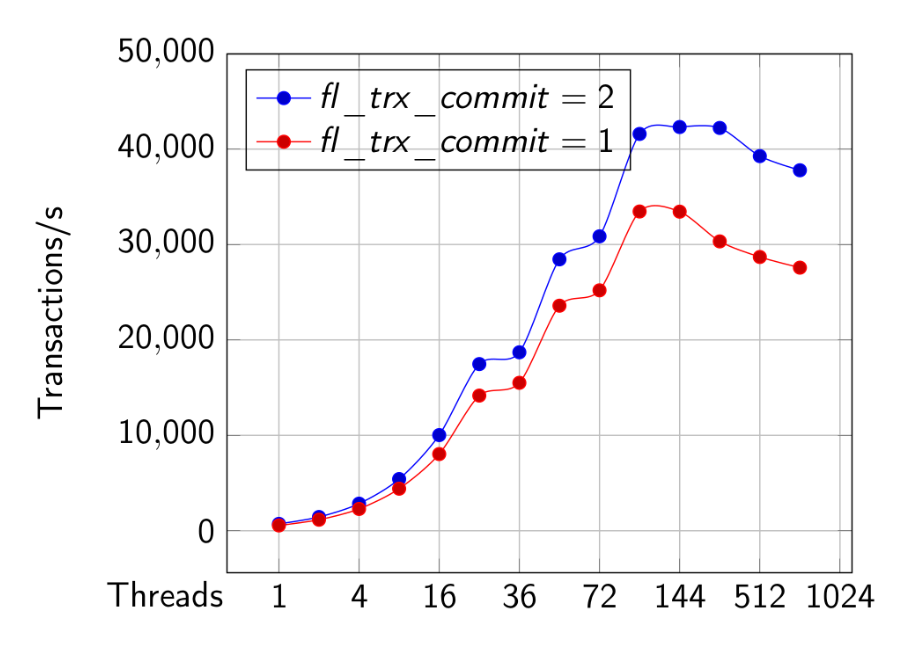
\includegraphics[width=0.5\textwidth]{mysql-scaling.png}
    \caption{Transactions/sec }
\end{figure}

\begin{itemize}
    \item Processing power of 16-64 = slightly less then 4x
    \item Real performance: 2.3x
    \item = scaling up: add more processing power to the system
\end{itemize}

\subsubsection{ElasticSearch Scaling: distributed system}

\begin{figure}[H]
    \centering
    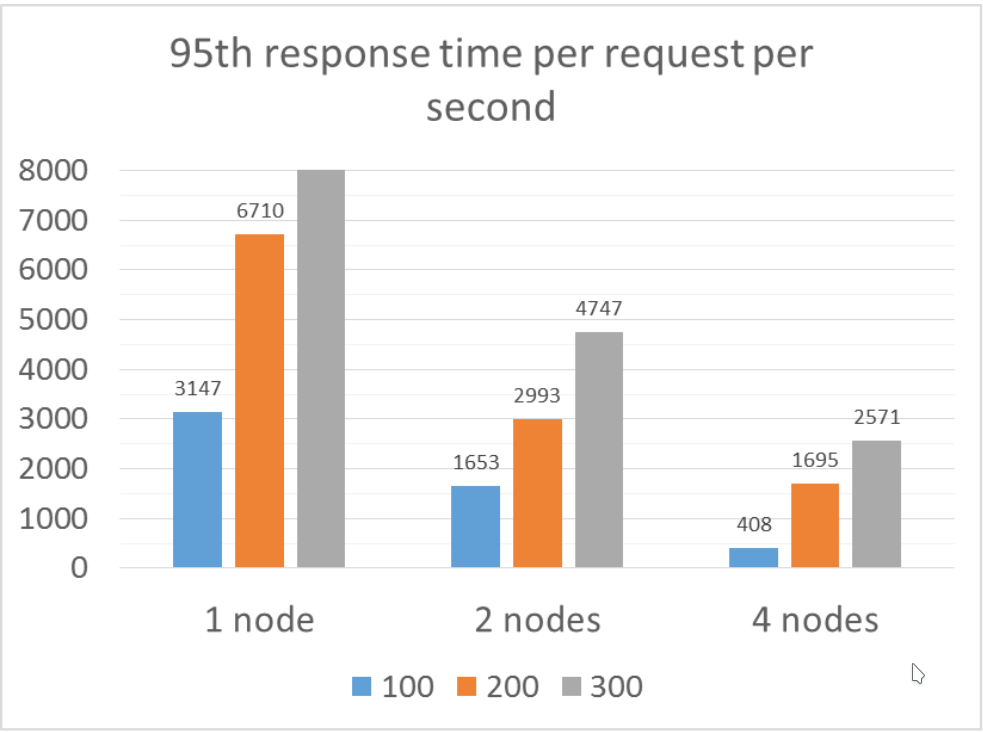
\includegraphics[width=0.5\textwidth]{elasticsearch-scaling.png}
    \caption{Response time per request}
\end{figure}

\begin{itemize}
    \item Scaling out: add more servers to your data system
\end{itemize}

\subsubsection{Professional architecture (Dev oriented)}

\begin{figure}[H]
    \centering
    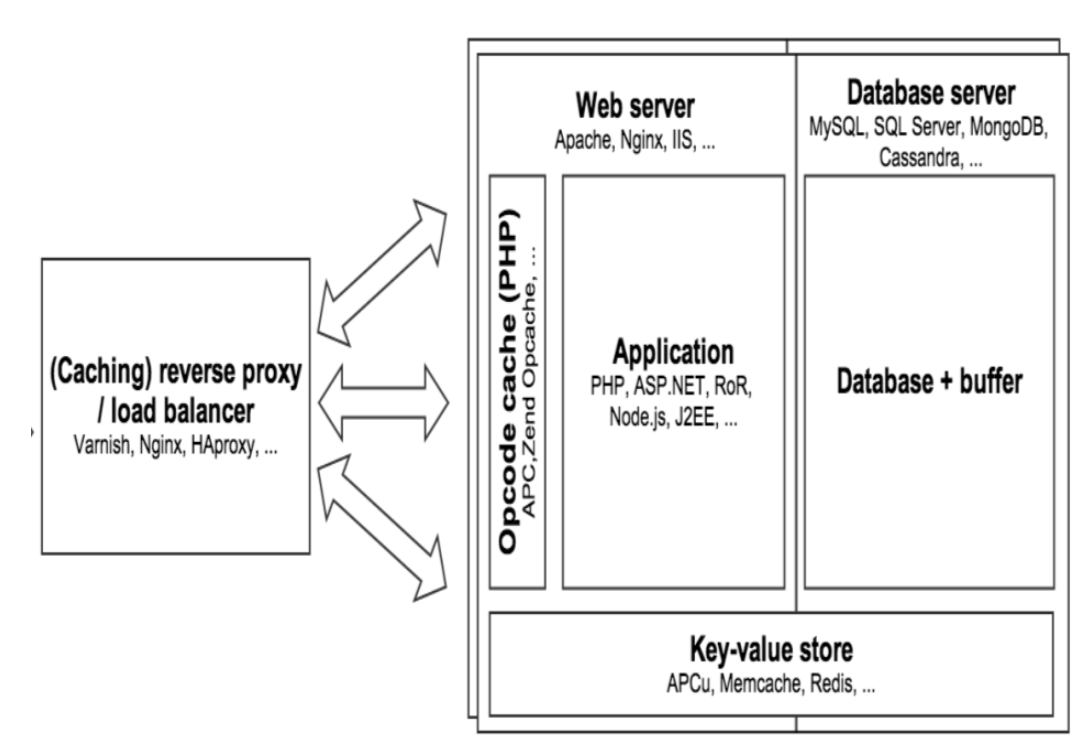
\includegraphics[width=0.5\textwidth]{professional-architecture.png}
    \caption{Professional architecture diagram}
\end{figure}


\begin{itemize}
    \item \bold{Reverse proxy / Load balancer:} improves scalability
    \item \bold{Opcode/app/Webserver:} webservice + API
    \item \bold{Key-value store:} `caching layer'
    \item \bold{Database server:} distributed storage system + relational database
\end{itemize}

\subsubsection{Time series Distributed database (OpenTSDB, InfluxDB)}

\begin{figure}[H]
    \centering
    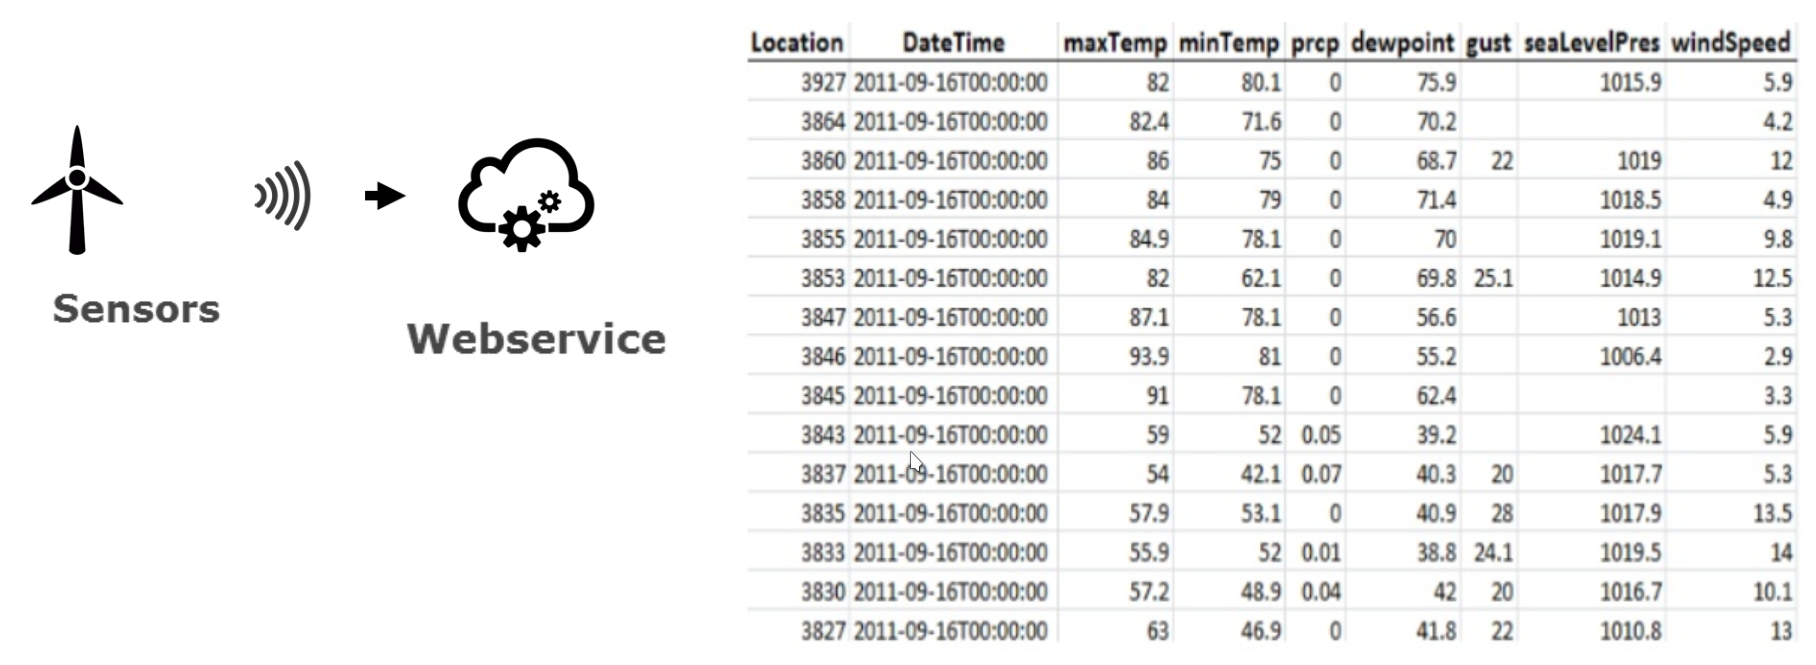
\includegraphics[width=0.5\textwidth]{time-series-distributed-db.png}
    \caption{Data from windmill sensors. Most sensors log about every second}
\end{figure}

\begin{itemize}
    \item Losing data is not that big a problem
    \item Massive amount of data to write 
\end{itemize}

\subsection{Scalability \& application performance management}

Response times and percentiles rule the web

\subsubsection{The need for speed: some insights from Google}

\begin{itemize}
    \item Speed is a ranking factor
    \item When your site has high response times, less URLs will be crawled from your site
    \item 53\% of visits are abandoned if a site takes longer than 3 seconds to load
    \item Slow websites will be labeled by Google Chrome
\end{itemize}

\subsubsection{Response times for websites}

\begin{itemize}
    \item \bold{Ideal:} "blink of an eye" is 300-400 ms
    \item \bold{Excellent:} 500ms to 1.5 seconds at most
    \item \bold{Barely acceptable:} 3 seconds
\end{itemize}

Response time = Network latency + processing

\begin{itemize}
    \item 2.9 seconds is faster than 50\% of the web
    \item 1.7 seconds is faster than 75\% of the web
    \item 0.8 seconds is faster than 94\% of the web
\end{itemize}

\subsubsection{4 components of network latency}

\begin{figure}[H]
    \centering
    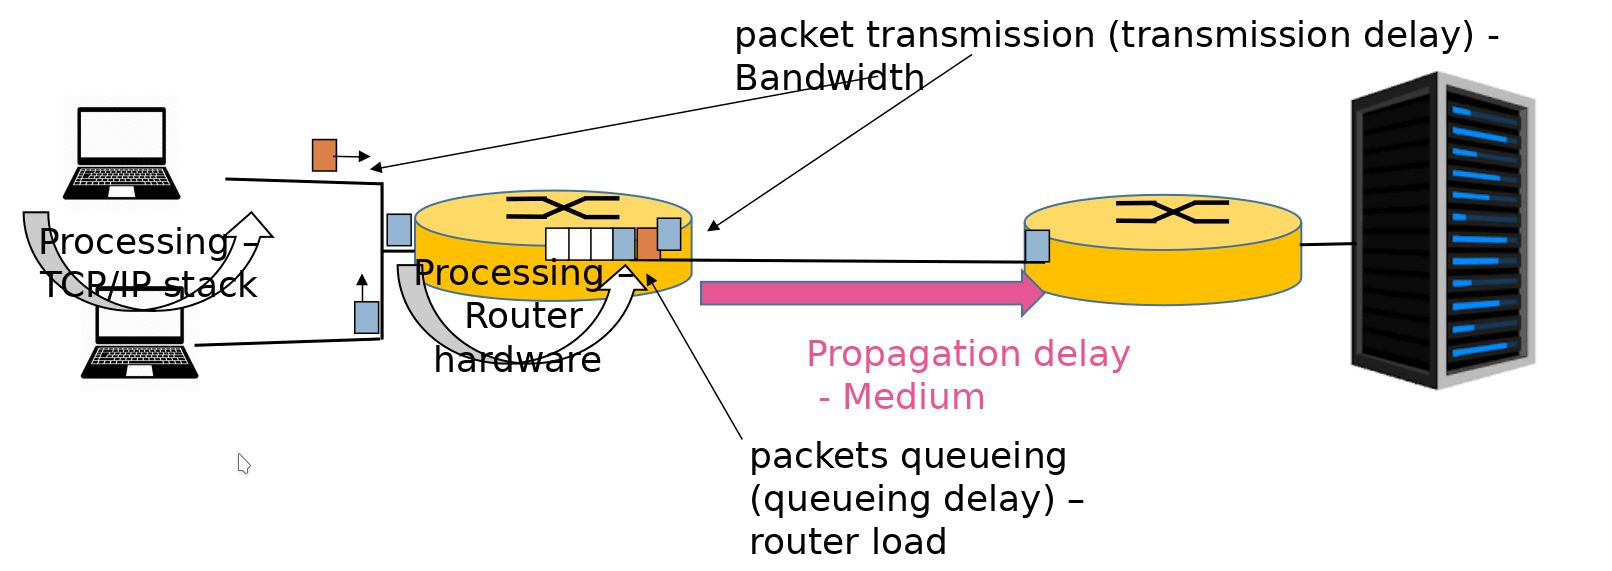
\includegraphics[width=0.5\textwidth]{network-latency.png}
    \caption{Network latency diagram}
\end{figure}

\begin{itemize}
    \item Processing delay
    \begin{itemize}
        \item Processing network software stack (TCP/IP layers)
        \item Routing decisions
    \end{itemize}
    \item Transmission delay
    \begin{itemize}
        \item Bits on physical link (Bandwidth plays a big role, ex: 1Gbit/s)
    \end{itemize}
    \item Propagation delay
    \begin{itemize}
        \item Speed of EM signals in fiber: 200.000 km/s (67\% of lightspeed)
        \item Changes with distance and medium (Copper: 64\% of lightspeed)
    \end{itemize}
    \item Queing delay
    \begin{itemize}
        \item Time spent in router \& NIC buffers
    \end{itemize}
\end{itemize}

\subsubsection{TCP Congestion Window - slow start}

\begin{itemize}
    \item Network congestion = a network node or link is carrying more data than it can handle
    \item The internet is built around dropped packages
\end{itemize}

\begin{figure}[H]
    \centering
    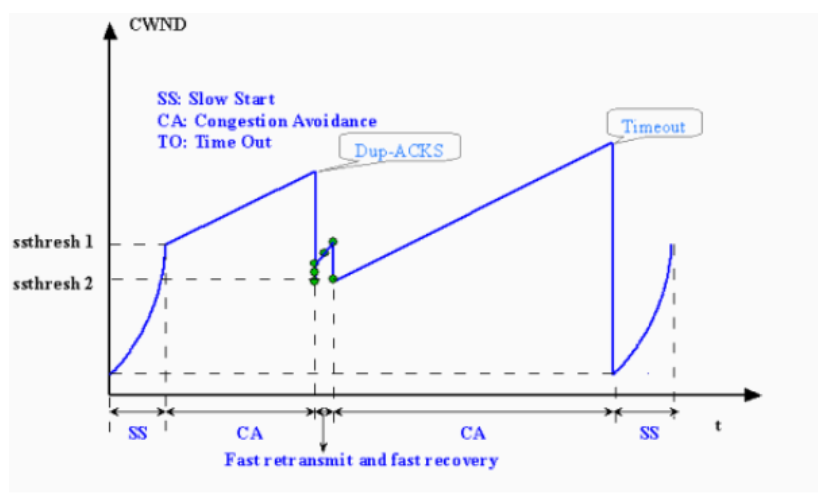
\includegraphics[width=0.5\textwidth]{tcp-congestion-window.png}
    \caption{TCP Congestion window}
\end{figure}

\begin{itemize}
    \item 4-8-16-32 TCP segments (Win 2008, Win7)
    \item 10-20-40 (Linux 2.6+, Windows Server 2016 / Windows 10)
\end{itemize}

\begin{figure}[H]
    \centering
    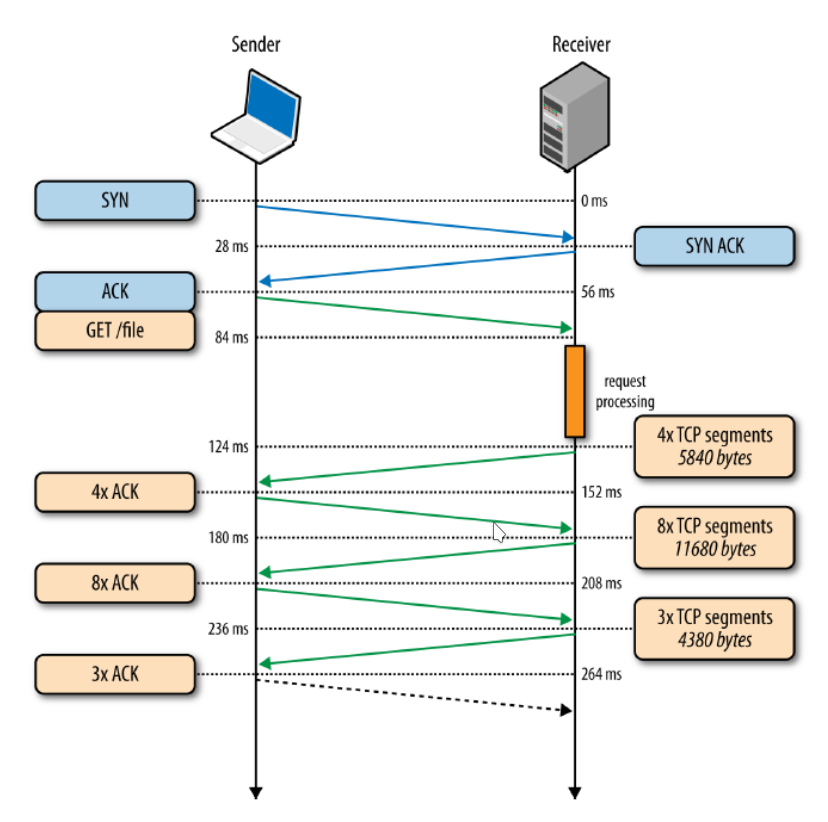
\includegraphics[width=0.5\textwidth]{tcp-handshakes.png}
    \caption{Because of many handshakes, there is a lot of latency}
\end{figure}

\begin{itemize}
    \item Solution: KeepAlive of a HTTP Persistent Connection
    \begin{itemize}
        \item Only one 3-way handshake for many requests
        \item Lower network \& CPU load
        \item Lower response times
        \item \bold{Downside}: more connections open $\Rightarrow$ more memory, more connection failures, app crashing, \dots
    \end{itemize}
\end{itemize}

\begin{itemize}
    \item Measure parallel requests of a website using \url{https://www.webpagetest.org/}
    \item Get a waterfall view of a webpage
\end{itemize}

\subsubsection{Long tail latency}

\begin{figure}[H]
    \centering
    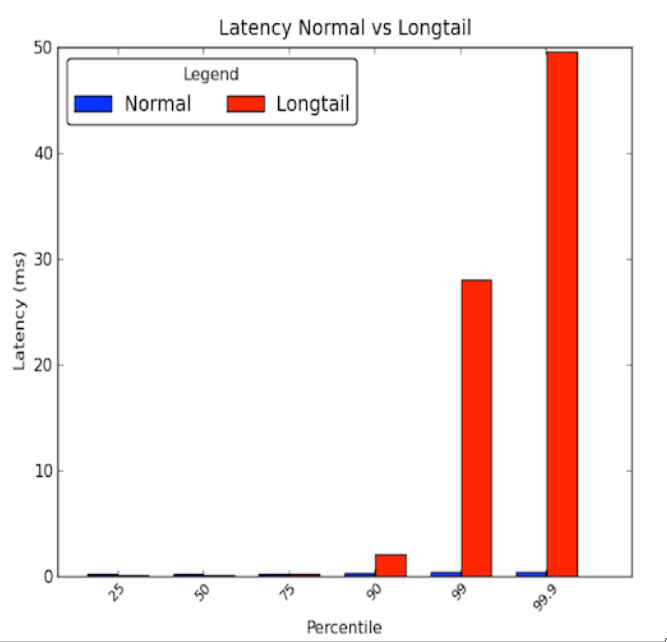
\includegraphics[width=0.5\textwidth]{long-tail-latency.png}
    \caption{Long tail latency vs Normal latency}
\end{figure}


\begin{itemize}
    \item Average = useless
    \item Long tail latency = 99th percentile
    \begin{itemize}
        \item To be experienced by a lot more than 1\% of users!
    \end{itemize}
    \item Best customers encounter highest percentiles
    \item URL consists of many requests
\end{itemize}

\subsection{Conclusion}

\begin{itemize}
    \item Our goal is RAMS (or RASS)
    \item Many data models \& stores: transactional, timeseries, text search
    \item Website 99th percentile + DNS + TCP $\Rightarrow$ < 2s response time
    \begin{itemize}
        \item Efficient caching
        \item Think about your architecture (infrastructure + software) before coding
    \end{itemize}
\end{itemize}

\section{Professional storage}

\subsection{Cloud MIPS}

\begin{figure}[H]
    \centering
    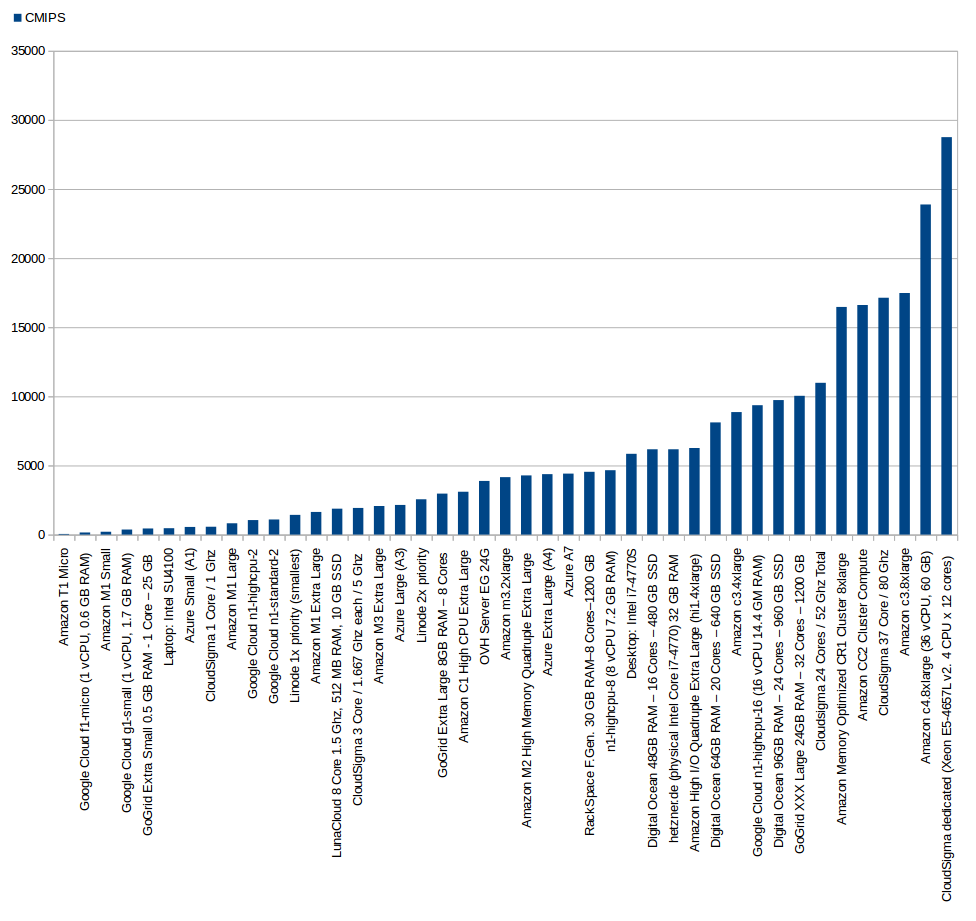
\includegraphics[width=0.5\textwidth]{mips.png}
    \caption{MIPS = Million Instructions Per Second}
\end{figure}

\subsection{Latency vs storage space pyramid}

\begin{figure}[H]
    \centering
    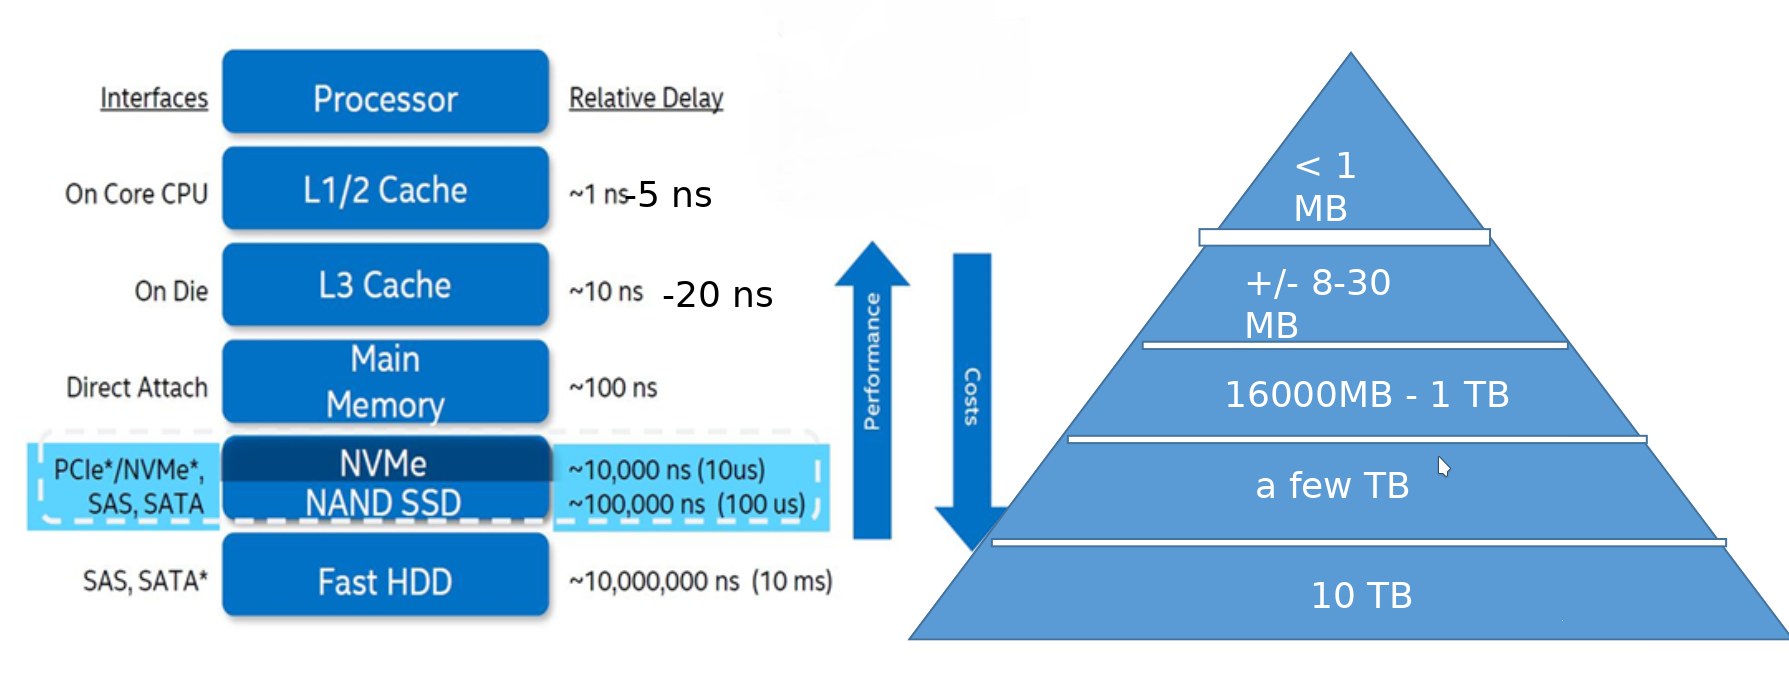
\includegraphics[width=0.5\textwidth]{latency-vs-storage-space-pyramid.png}
    \caption{The higher the performance, the higher the cost per byte of storage}
\end{figure}

\subsection{Storage media}

\subsubsection{Magnetic disks}

\begin{figure}[H]
    \centering
    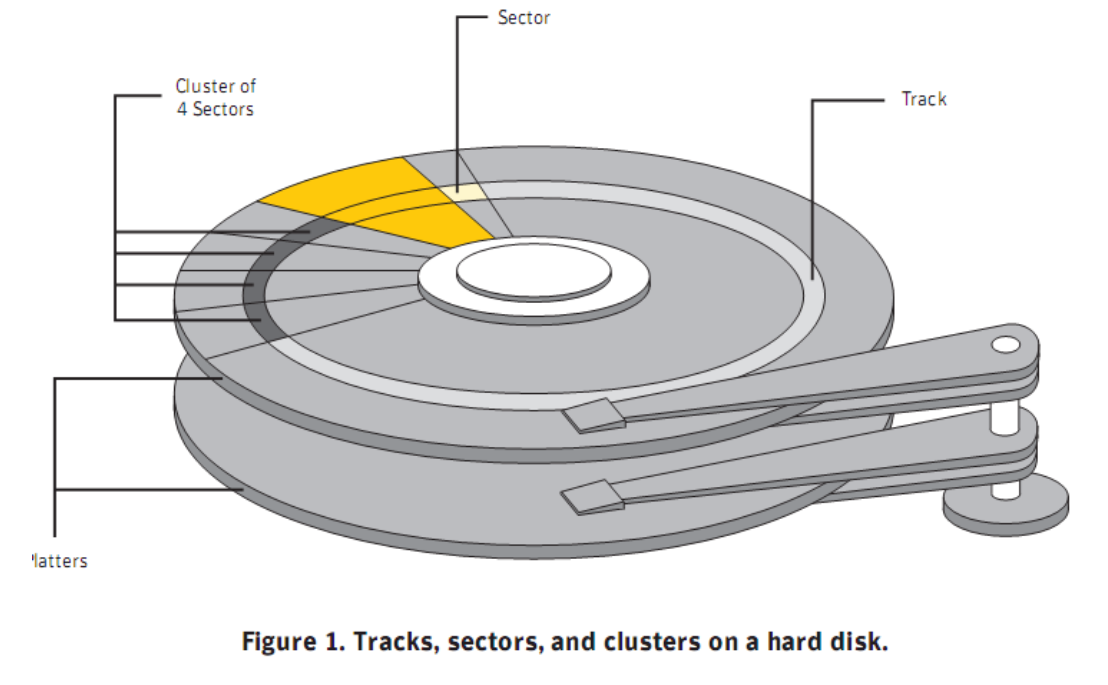
\includegraphics[width=0.5\textwidth]{magnetic-disks.png}
    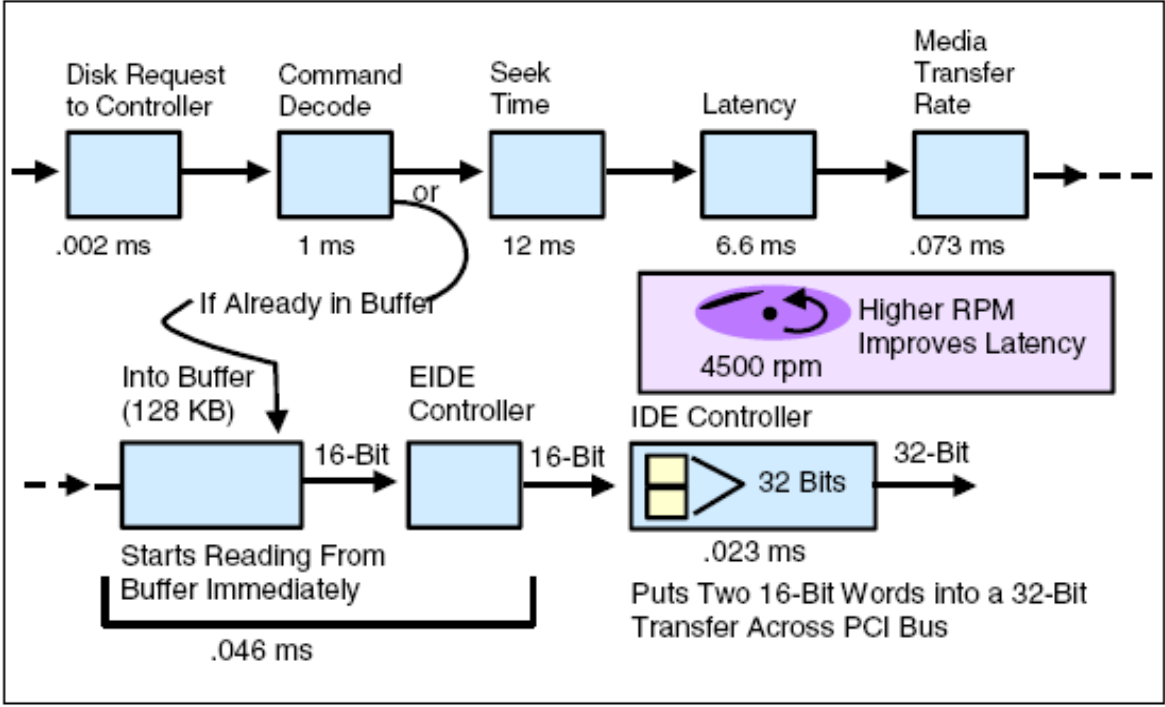
\includegraphics[width=0.4\textwidth]{magnetic-disks-performance.png}
    \caption{Massive capacity but mechanical latency}
\end{figure}

\begin{itemize}
    \item Seek time and latency are the key bottlenecks
    \item Need large quantity of disks for good server performance
\end{itemize}

\subsubsection{Flash (NAND) / SSDs}

\begin{figure}[H]
    \centering
    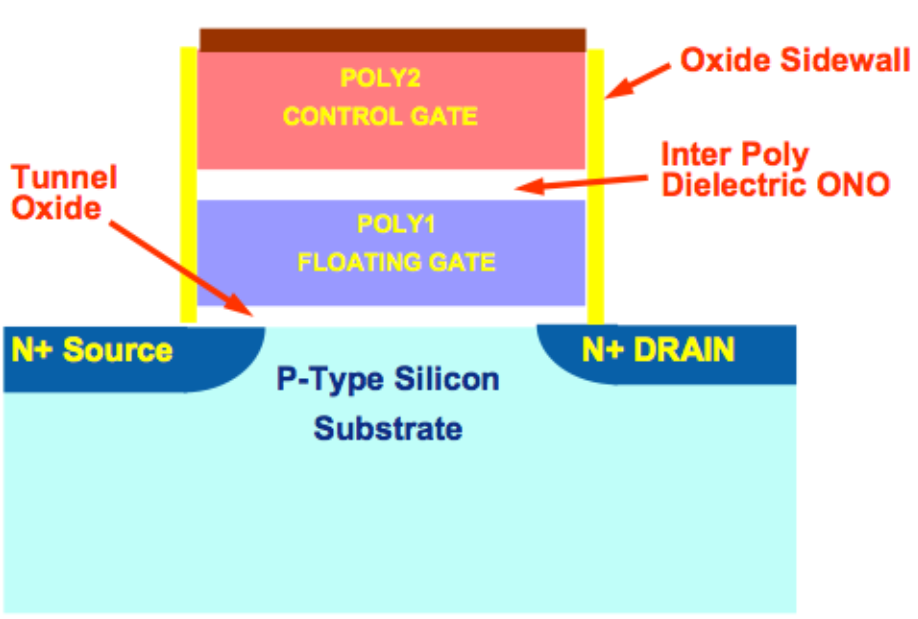
\includegraphics[width=0.5\textwidth]{flash-nand.png}
    \caption{Flash storage}
\end{figure}

\begin{itemize}
    \item NAND = MOSFET + floating gate
    \item Voltage between control gate and N+ : electrons in floating gate
    \item This works very quickly
\end{itemize}

\subsubsection{Big difference between read and writing}

\begin{figure}[H]
    \centering
    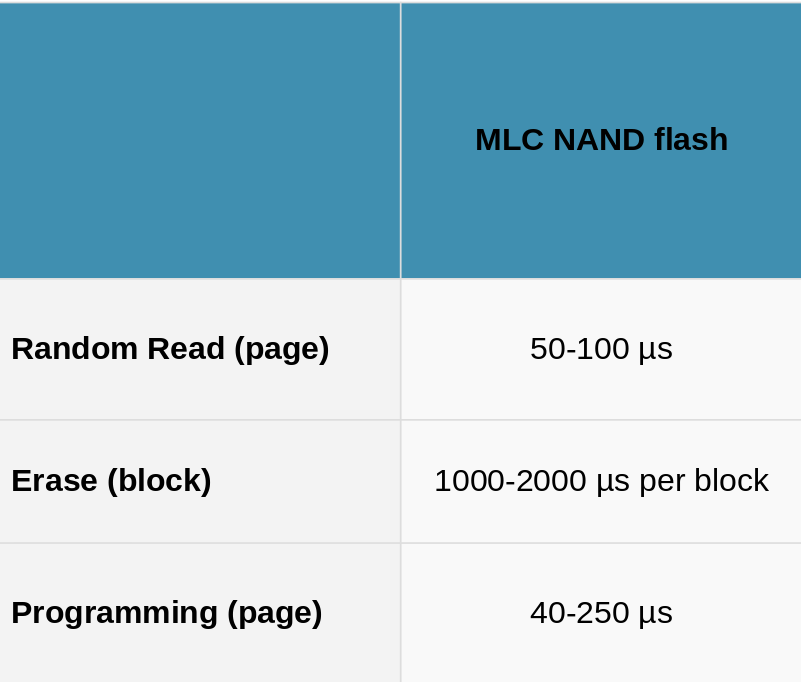
\includegraphics[width=0.5\textwidth]{nand-read-write.png}
    \caption{}
\end{figure}

\begin{itemize}
    \item Limited number of writes
    \item Slow block write
    \item Limited "normal" write (programming)
\end{itemize}

\subsubsection{IOPS vs Bandwidth}

\begin{itemize}
    \item Transactions \& virtualized workloads: lots of random access
    \item Timeseries fileserving: mostly sequential
    \item HDD: random performance can be extremely low to medium 
    \item IOPS = Input/Output Operations Per Second
\end{itemize}

\begin{figure}[H]
    \centering
    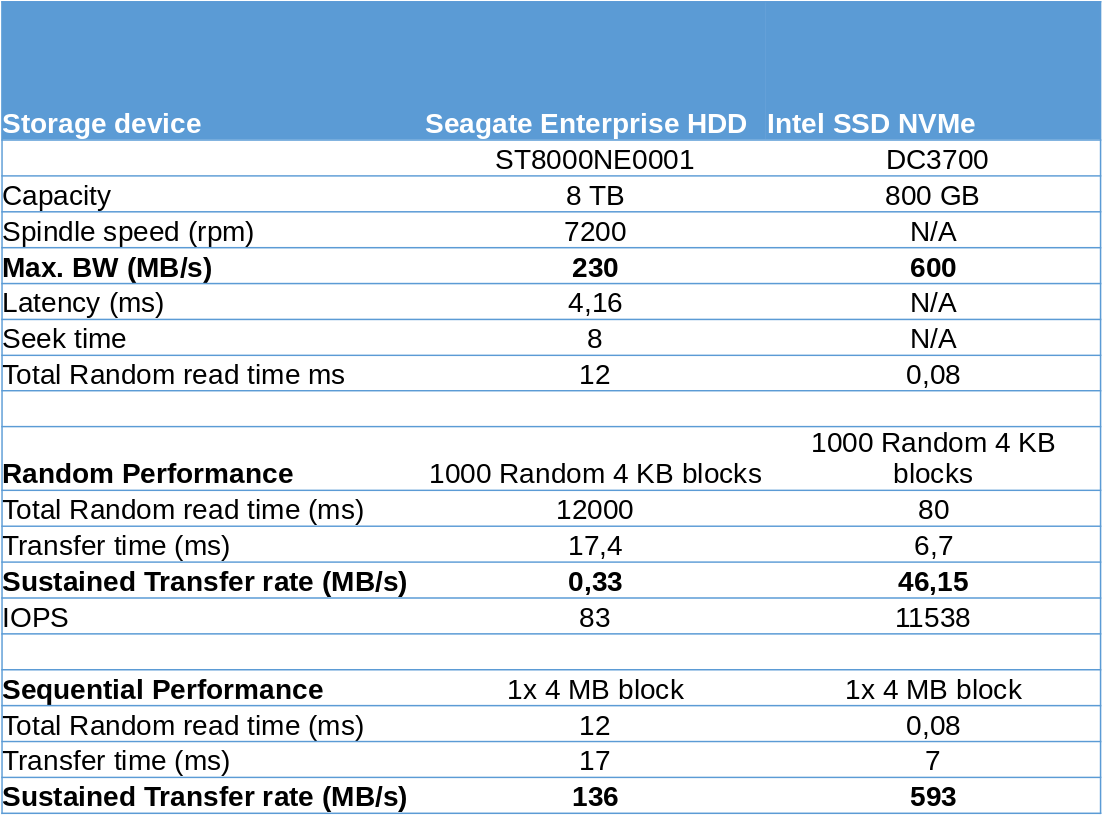
\includegraphics[width=0.5\textwidth]{storage-device-comparison.png}
    \caption{An enterprise HDD vs an NVME SSD}
\end{figure}

\subsubsection{Storage options}

\begin{figure}[H]
    \centering
    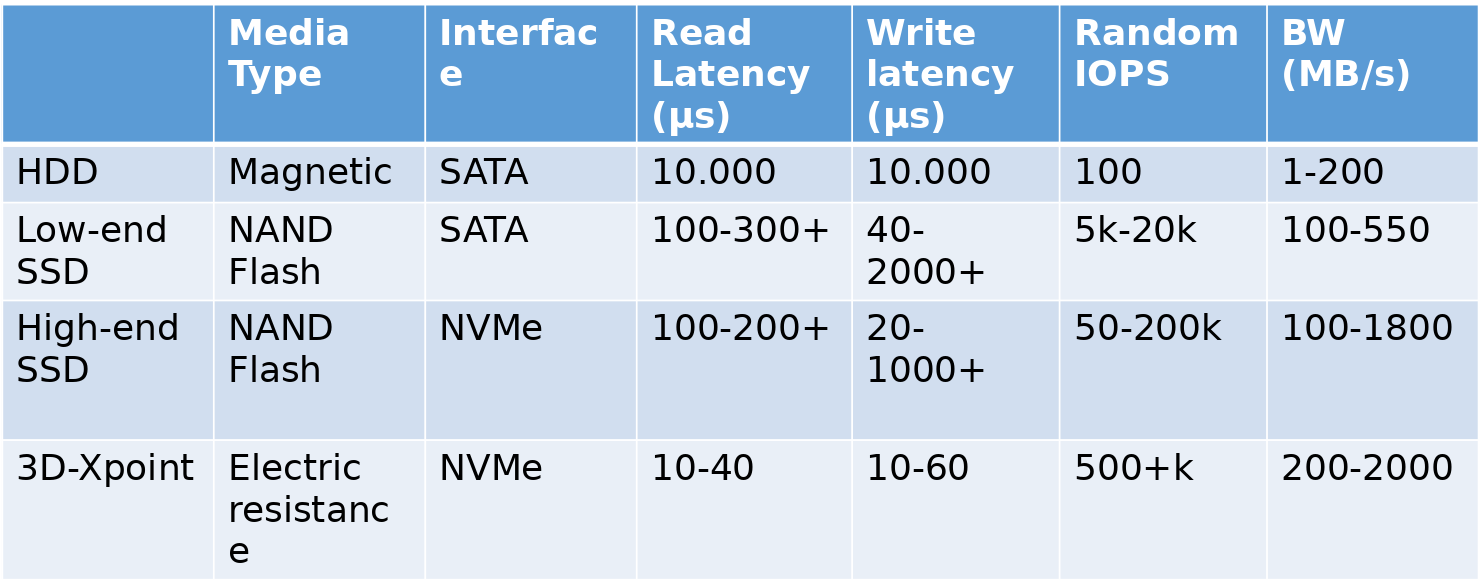
\includegraphics[width=0.6\textwidth]{storage-options.png}
    \caption{Storage options}
\end{figure}

\begin{figure}[H]
    \centering
    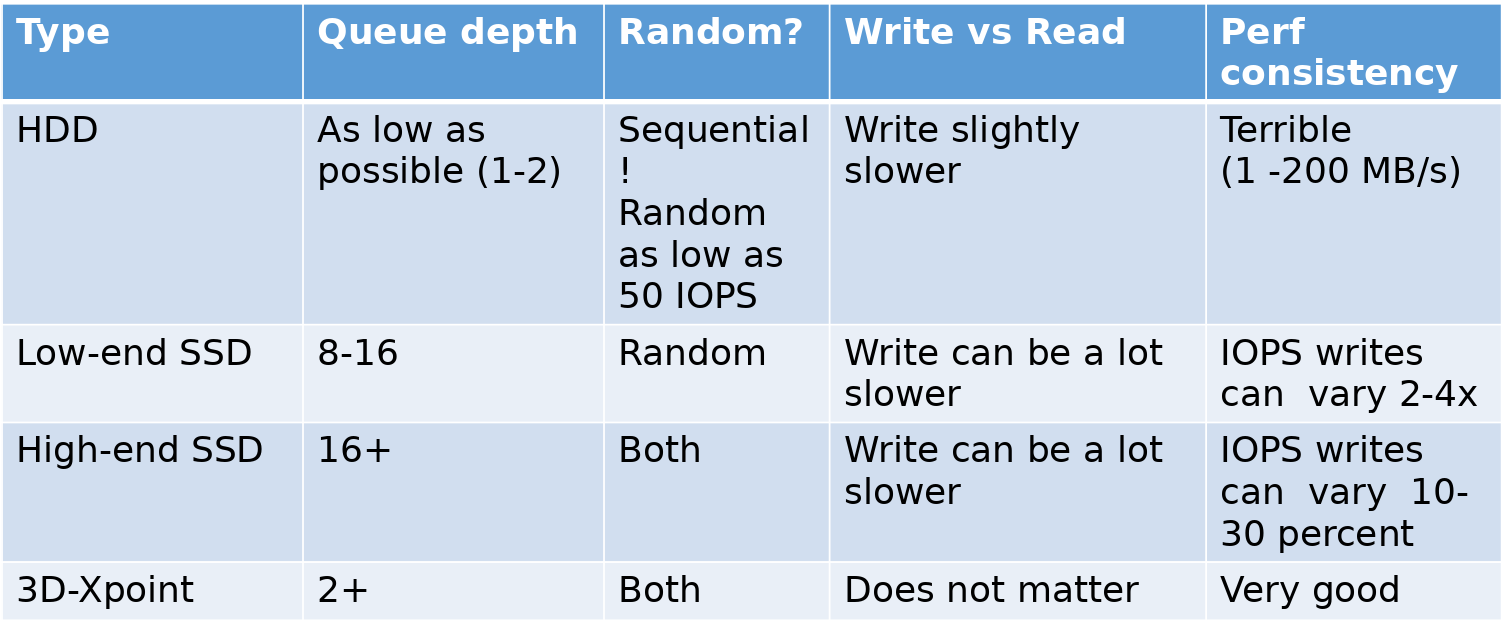
\includegraphics[width=0.6\textwidth]{performance-conditions.png}
    \caption{Performance Conditions}
\end{figure}


\subsection{Professional Storage Topology}




\end{document}